\documentclass[11pt,a4paper]{article}

\usepackage[margin=1in]{geometry}
\usepackage{amsmath,amssymb,amsfonts,mathtools}
\usepackage{bm}
\usepackage{physics}
\usepackage{tikz}
\usetikzlibrary{arrows.meta, positioning, fit, shapes.geometric, calc, decorations.pathmorphing, backgrounds}
\usepackage{caption}
\usepackage{subcaption}
\usepackage{array}
\usepackage{booktabs}
\usepackage{enumitem}
\usepackage{xcolor}
\usepackage{listings}
\usepackage[most]{tcolorbox}
\usepackage{hyperref}
\usepackage{fancyhdr}
\usepackage{graphicx}
\usepackage{float}

% ============================================================================
% COLOR PALETTE
% ============================================================================
\definecolor{drakeblue}{RGB}{30,90,180}
\definecolor{drakecyan}{RGB}{0,150,180}
\definecolor{drakegreen}{RGB}{40,140,60}
\definecolor{darkred}{RGB}{180,30,30}
\definecolor{resultbg}{RGB}{230,255,230}
\definecolor{resultbar}{RGB}{40,140,60}
\definecolor{warnbg}{RGB}{255,245,220}
\definecolor{warnbar}{RGB}{200,140,0}
\definecolor{lightgray}{RGB}{245,245,245}

% --- Equation-after-code box ---
\definecolor{eqboxbg}{RGB}{236,244,255}
\definecolor{eqboxbar}{RGB}{45,95,165}
\definecolor{eqboxlabel}{RGB}{35,80,145}

\newtcolorbox{codemath}{%
    enhanced,
    breakable,
    colback=eqboxbg,
    colframe=eqboxbar,
    boxrule=0pt,
    leftrule=3.5pt,
    arc=0pt,
    outer arc=0pt,
    top=8pt,
    bottom=8pt,
    left=10pt,
    right=10pt,
    before skip=4pt,
    after skip=10pt,
    before upper={\noindent\textcolor{eqboxlabel}{\sffamily\bfseries\small%
        \raisebox{0.3pt}{$\blacktriangleright$}~Equations implemented by the above code}\par\medskip},
}

% --- Result highlight box ---
\newtcolorbox{resultbox}[1][]{%
    enhanced,
    breakable,
    colback=resultbg,
    colframe=resultbar,
    boxrule=0pt,
    leftrule=4pt,
    arc=0pt,
    outer arc=0pt,
    top=8pt,
    bottom=8pt,
    left=10pt,
    right=10pt,
    before skip=6pt,
    after skip=10pt,
    title={\textcolor{resultbar}{\sffamily\bfseries {\large $\checkmark$}~Key Result} #1},
}

% --- Warning box ---
\newtcolorbox{warnbox}[1][]{%
    enhanced,
    breakable,
    colback=warnbg,
    colframe=warnbar,
    boxrule=0pt,
    leftrule=4pt,
    arc=0pt,
    outer arc=0pt,
    top=8pt,
    bottom=8pt,
    left=10pt,
    right=10pt,
    before skip=6pt,
    after skip=10pt,
    title={\textcolor{warnbar}{\sffamily\bfseries {\large $\triangle$}~Important} #1},
}

% --- Architecture box ---
\newtcolorbox{archbox}[1][]{%
    enhanced,
    breakable,
    colback=blue!3,
    colframe=drakeblue,
    boxrule=0.8pt,
    arc=3pt,
    outer arc=3pt,
    top=8pt,
    bottom=8pt,
    left=10pt,
    right=10pt,
    before skip=8pt,
    after skip=10pt,
    title={\textcolor{drakeblue}{\sffamily\bfseries #1}},
}

% --- Python code style ---
\definecolor{pybg}{RGB}{248,252,248}
\definecolor{pyframe}{RGB}{160,190,160}
\definecolor{pykw}{RGB}{0,110,0}
\definecolor{pycmt}{RGB}{100,100,100}
\definecolor{pystr}{RGB}{160,32,240}

\lstdefinestyle{python}{
    language=Python,
    basicstyle=\small\ttfamily,
    keywordstyle=\color{pykw}\bfseries,
    commentstyle=\color{pycmt}\itshape,
    stringstyle=\color{pystr},
    backgroundcolor=\color{pybg},
    frame=single,
    rulecolor=\color{pyframe},
    framesep=4pt,
    xleftmargin=6pt,
    xrightmargin=6pt,
    breaklines=true,
    breakatwhitespace=false,
    showstringspaces=false,
    tabsize=4,
    captionpos=b,
    numbers=left,
    numberstyle=\tiny\color{gray},
    aboveskip=8pt,
    belowskip=4pt,
    morekeywords={np,self,True,False,None,float},
}
\lstset{style=python}

% ============================================================================
% HEADER / FOOTER
% ============================================================================
\pagestyle{fancy}
\fancyhf{}
\fancyhead[L]{\small\textcolor{drakeblue}{\textbf{PyDrake Computed-Torque Implementation}}}
\fancyhead[R]{\small\textcolor{gray}{Cup Manipulator Tendon}}
\fancyfoot[C]{\thepage}
\renewcommand{\headrulewidth}{0.5pt}
\renewcommand{\headrule}{\hbox to\headwidth{\color{drakeblue}\leaders\hrule height \headrulewidth\hfill}}

% ============================================================================
% COMMANDS
% ============================================================================
\newcommand{\rp}{r_{\mathrm{p}}}
\newcommand{\bq}{\bm{q}}
\newcommand{\bdq}{\dot{\bm{q}}}
\newcommand{\bddq}{\ddot{\bm{q}}}
\newcommand{\btau}{\bm{\tau}}
\newcommand{\bM}{\bm{M}}
\newcommand{\bh}{\bm{h}}
\newcommand{\bJ}{\bm{J}}
\newcommand{\bx}{\bm{x}}

\title{%
    \textcolor{drakeblue}{\rule{\linewidth}{1.5pt}}\\[0.4cm]
    {\Huge\bfseries Computed-Torque Controller}\\[0.3cm]
    {\Large\textcolor{drakecyan}{Cable-Driven 2R Planar Manipulator --- PyDrake Implementation}}\\[0.2cm]
    \textcolor{drakeblue}{\rule{\linewidth}{1.5pt}}
}
\author{Isaac Sim Robotics Project}
\date{April 2026}

\begin{document}
\maketitle
\thispagestyle{empty}

% ============================================================================
\section*{Key Results at a Glance}
% ============================================================================

\begin{resultbox}
\begin{itemize}[leftmargin=1.5em]
    \item \textbf{Tracking RMS error}: $< 1$\,mm on 20\,mm $\times$ 160\,mm rectangle trajectory
    \item \textbf{Controller}: Inverse-dynamics (computed torque) with joint-space PD + feedforward
    \item \textbf{Closed-loop bandwidth}: $\omega_n = \sqrt{K_p} \approx 20$\,rad/s, $\zeta = 1.0$ (critically damped)
    \item \textbf{Simulation framework}: PyDrake MultibodyPlant --- analytical dynamics, Meshcat 3D visualization
    \item \textbf{Cable actuation}: Joint-2 driven via HTD\,5M belt with pulley radius $\rp = 47.7$\,mm
    \item \textbf{Architecture}: Two-plant Drake pattern (physics + controller) with diagram-based signal routing
\end{itemize}
\end{resultbox}

\tableofcontents
\newpage

% ============================================================================
\section{Algorithm Overview}
\label{sec:overview}
% ============================================================================

This section gives the top-level picture before the detailed derivations that follow.

\subsection{What the Simulation Actually Does}

The simulation runs a \textbf{single Drake \texttt{MultibodyPlant}} loaded from a URDF with \textbf{two revolute joints}.  A computed-torque controller (a Drake \texttt{LeafSystem}) reads the plant state, computes joint torques via inverse dynamics, and writes them back to the plant's actuation port.  The closed-loop runs at 500\,Hz (2\,ms timestep).

\begin{archbox}{Core Control Loop}
\begin{center}
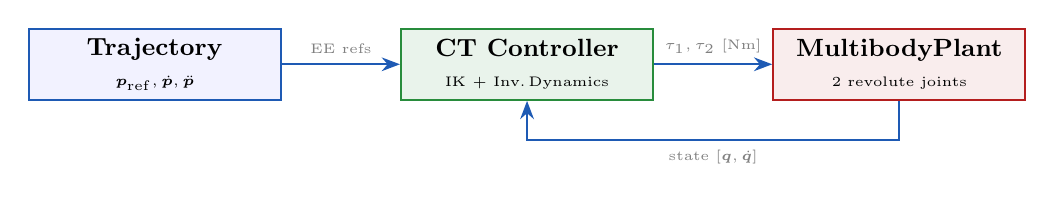
\begin{tikzpicture}[
    node distance=0.6cm and 1.8cm,
    block/.style={rectangle, draw=drakeblue, thick, fill=blue!5,
                  minimum height=0.9cm, minimum width=3.2cm, align=center, font=\small},
    arr/.style={-Stealth, thick, drakeblue},
    port/.style={font=\tiny, text=gray},
]
    \node[block] (ref)  {\textbf{Trajectory}\\{\tiny $\bm{p}_{\mathrm{ref}}, \dot{\bm{p}}, \ddot{\bm{p}}$}};
    \node[block, right=1.5cm of ref, fill=drakegreen!10, draw=drakegreen] (ct) {\textbf{CT Controller}\\{\tiny IK + Inv.\,Dynamics}};
    \node[block, right=1.5cm of ct, fill=darkred!8, draw=darkred] (plant) {\textbf{MultibodyPlant}\\{\tiny 2 revolute joints}};

    \draw[arr] (ref) -- (ct) node[midway, above, port] {EE refs};
    \draw[arr] (ct) -- (plant) node[midway, above, port] {$\tau_1, \tau_2$ [Nm]};
    \draw[arr] (plant.south) -- ++(0,-0.5) -| (ct.south)
        node[pos=0.25, below, port] {state $[\bq, \dot{\bq}]$};
\end{tikzpicture}
\end{center}
\end{archbox}

\subsection{Algorithm Flow --- Step by Step}

Every simulation timestep the controller executes:

\begin{enumerate}[leftmargin=2em]
    \item \textbf{Read state} $(\bq, \dot{\bq})$ from the MultibodyPlant
    \item \textbf{Evaluate trajectory} $\to$ desired EE position $\bm{p}_{\mathrm{ref}}$, velocity $\dot{\bm{p}}_{\mathrm{ref}}$, acceleration $\ddot{\bm{p}}_{\mathrm{ref}}$
    \item \textbf{Inverse kinematics}: $\bm{p}_{\mathrm{ref}} \xrightarrow{\text{2R analytical}} \bq_{\mathrm{des}}$
    \item \textbf{Differential IK}: $\dot{\bm{p}}_{\mathrm{ref}} \xrightarrow{\bJ^{-1}} \dot{\bq}_{\mathrm{ref}}$, \quad $\ddot{\bm{p}}_{\mathrm{ref}} \xrightarrow{\bJ^{-1}} \ddot{\bq}_{\mathrm{ref}}$
    \item \textbf{PD + feedforward}: $\bm{a}_{\mathrm{des}} = \ddot{\bq}_{\mathrm{ref}} + K_p(\bq_{\mathrm{des}} - \bq) + K_d(\dot{\bq}_{\mathrm{ref}} - \dot{\bq})$
    \item \textbf{Inverse dynamics}: $\btau = \bM(\bq)\,\bm{a}_{\mathrm{des}} + \bh(\bq, \dot{\bq})$ \quad via Drake's \texttt{CalcInverseDynamics}
    \item \textbf{Saturate and apply}: $\btau_{\mathrm{clip}} = \mathrm{clip}(\btau, \pm\tau_{\max})$ $\to$ plant actuation port
\end{enumerate}

\subsection{What the Cable Is (and Isn't)}

\begin{warnbox}
\textbf{The cable/belt is NOT modeled as a physical element.}  The Drake \texttt{MultibodyPlant} contains only two rigid revolute joints---there is no spring, cable, or pulley in the physics simulation.  The belt is treated as a \textbf{rigid tendon}: an inextensible, massless transmission between motor and joint.
\end{warnbox}

The controller outputs \textbf{joint torques} $[\tau_1, \tau_2]$ in Nm, which are applied directly to the plant's actuation port.  There is no cable compliance, no pulley friction, and no belt elasticity in the dynamics.

Cable tensions appear in the code as a \textbf{post-hoc decomposition} for logging and feasibility checking:
\[
    F_{\mathrm{net}} = \frac{\tau_2}{r_p}, \qquad
    T_{\mathrm{green}} = \max(F_{\mathrm{net}}, 0), \qquad
    T_{\mathrm{red}} = \max(-F_{\mathrm{net}}, 0)
\]
This decomposition enforces the physical constraint that cables can only pull---if $T_{\mathrm{green}} > 0$ and $T_{\mathrm{red}} > 0$ simultaneously, the tendon assumption is violated.  But the plant simulation itself never sees cable tensions; it only receives $\tau_1, \tau_2$.

The cable \textbf{visualization} (coloured polylines in Meshcat) is likewise separate from the physics.  A headless \texttt{DrakeCablePlant} computes pulley tangent geometry via FK for rendering only.

\newpage

% ============================================================================
\section{Source File Architecture}
\label{sec:files}
% ============================================================================

This implementation spans six Python modules.  Each module has a distinct responsibility, and they compose through Drake's \texttt{DiagramBuilder} wiring pattern.

\subsection{File Dependency Map}

\begin{archbox}{Module Dependencies}
\begin{center}
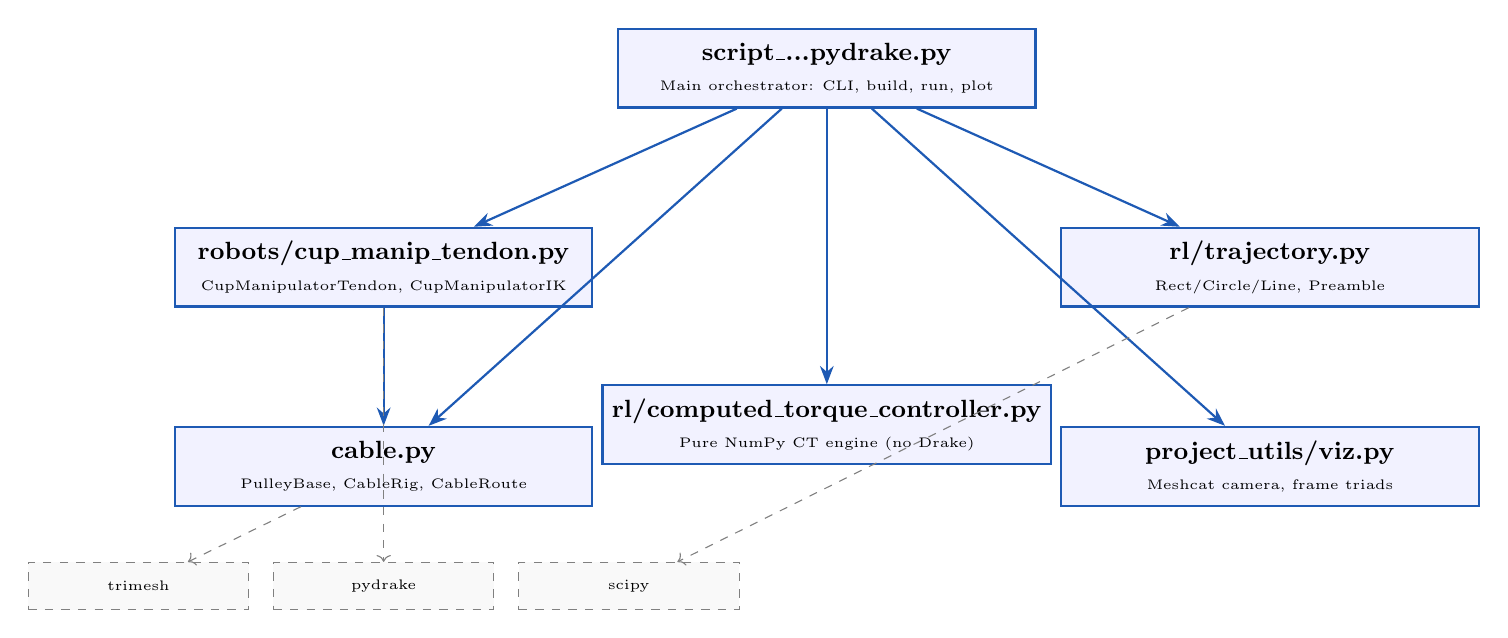
\begin{tikzpicture}[
    node distance=1.2cm and 2cm,
    mod/.style={rectangle, draw=drakeblue, thick, fill=blue!5,
                minimum height=1cm, minimum width=5.3cm, align=center, font=\small},
    lib/.style={rectangle, draw=gray, dashed, fill=gray!5,
                minimum height=0.6cm, minimum width=2.8cm, align=center, font=\tiny},
    arr/.style={-Stealth, thick, drakeblue},
]
    \node[mod] (main) {\textbf{script\_...pydrake.py}\\{\tiny Main orchestrator: CLI, build, run, plot}};

    \node[mod, below left=1.5cm and 0.3cm of main] (robot)
        {\textbf{robots/cup\_manip\_tendon.py}\\{\tiny CupManipulatorTendon, CupManipulatorIK}};

    \node[mod, below right=1.5cm and 0.3cm of main] (traj)
        {\textbf{rl/trajectory.py}\\{\tiny Rect/Circle/Line, Preamble}};

    \node[mod, below=3.5cm of main] (ct)
        {\textbf{rl/computed\_torque\_controller.py}\\{\tiny Pure NumPy CT engine (no Drake)}};

    \node[mod, below=1.5cm of robot] (cable)
        {\textbf{cable.py}\\{\tiny PulleyBase, CableRig, CableRoute}};

    \node[mod, below=1.5cm of traj] (viz)
        {\textbf{project\_utils/viz.py}\\{\tiny Meshcat camera, frame triads}};

    \draw[arr] (main) -- (robot);
    \draw[arr] (main) -- (traj);
    \draw[arr] (main) -- (ct);
    \draw[arr] (main) -- (viz);
    \draw[arr] (robot) -- (cable);
    \draw[arr] (main) -- (cable);

    \node[lib, below=0.7cm of cable] (drake) {pydrake};
    \node[lib, right=0.3cm of drake] (scipy) {scipy};
    \node[lib, left=0.3cm of drake] (trimesh) {trimesh};

    \draw[->, dashed, gray] (robot) -- (drake);
    \draw[->, dashed, gray] (cable) -- (trimesh);
    \draw[->, dashed, gray] (traj) -- (scipy);
\end{tikzpicture}
\end{center}
\end{archbox}

\subsection{Module Responsibilities}

\begin{table}[H]
\centering
\caption{Source file roles and key exports.}
\begin{tabular}{p{5.8cm}p{8cm}}
\toprule
\textbf{File} & \textbf{Key Exports / Role} \\
\midrule
\texttt{script\_...\_pydrake.py} ($\sim$1600 lines) &
    \texttt{IKPDSimulation}, \texttt{ComputedTorqueSimulation}, CLI parser, \texttt{\_SIM\_REGISTRY} dispatch \\
\texttt{robots/cup\_manipulator\_tendon.py} ($\sim$500) &
    \texttt{CupManipulatorTendon} (URDF loading, FK, weld, actuators), \texttt{CupManipulatorIK} (2R analytical IK, Jacobians) \\
\texttt{rl/computed\_torque\_controller.py} ($\sim$170) &
    \texttt{ComputedTorqueController.compute()}, \texttt{ik\_to\_joint\_space\_references()} --- pure NumPy, engine-agnostic \\
\texttt{rl/trajectory.py} ($\sim$300) &
    \texttt{RectTrajectory}, \texttt{CircleTrajectory}, \texttt{LineTrajectory}, \texttt{MoveToStartSpline}, \texttt{PreambleTrajectorySource} \\
\texttt{cable.py} ($\sim$800) &
    \texttt{PulleyBase} hierarchy, \texttt{CableRig}, \texttt{CableRoute}, \texttt{CableSpring}, tangent geometry \\
\texttt{project\_utils/viz.py} ($\sim$200) &
    \texttt{set\_meshcat\_camera\_spherical()}, \texttt{add\_frames\_to\_meshcat()}, frame triads \\
\bottomrule
\end{tabular}
\end{table}

\subsection{Design Principle: Engine-Agnostic Core}

A key architectural decision is the separation between \textbf{engine-agnostic} and \textbf{engine-specific} modules:

\begin{itemize}[leftmargin=2em]
    \item \texttt{rl/computed\_torque\_controller.py} uses \textbf{only NumPy}---no Drake imports.  It accepts $\bM$, $\bh$, and state vectors as plain arrays.  This allows the \emph{same controller} to run in both PyDrake and Isaac Sim.
    \item \texttt{rl/trajectory.py} uses \textbf{only SciPy}---no Drake imports.  Trajectories are portable across simulation engines.
    \item \texttt{robots/cup\_manipulator\_tendon.py} and the main script are Drake-specific, using \texttt{MultibodyPlant}, \texttt{LeafSystem}, and \texttt{DiagramBuilder}.
    \item \texttt{cable.py} uses Drake \texttt{MultibodyPlant} only for forward kinematics (a headless plant); the tangent-line geometry is pure NumPy.
\end{itemize}

\subsection{Import Graph --- Main Script}

The main script imports are organized by layer:

\begin{lstlisting}[caption={Import structure of the main simulation script.}]
# --- Engine layer (Drake) ---
from pydrake.all import (
    DiagramBuilder, Simulator, StartMeshcat,
    MultibodyPlant, Parser, AddMultibodyPlantSceneGraph,
    MeshcatVisualizer, MeshcatVisualizerParams, Role,
    LogVectorOutput,            # data logging
    ConstantVectorSource,       # trajectory sources
    RigidTransform, RotationMatrix,
)

# --- Robot layer ---
from robots.cup_manipulator_tendon import CupManipulatorTendon

# --- Engine-agnostic controller ---
from rl.computed_torque_controller import (
    ComputedTorqueController, ik_to_joint_space_references)

# --- Engine-agnostic trajectory ---
from rl.trajectory import (
    RectTrajectory, CircleTrajectory, LineTrajectory,
    PreambleTrajectorySource, build_move_to_start)

# --- Cable geometry ---
from cable import DrakeCablePlant, CableRig

# --- Visualization ---
from project_utils.viz import (
    set_meshcat_camera_spherical, add_frames_to_meshcat)
\end{lstlisting}

\newpage

% ============================================================================
\section{System Description}
% ============================================================================

\subsection{Physical Robot}

The cable-driven cup manipulator is a \textbf{2-DOF planar revolute-revolute (2R)} arm:

\begin{itemize}[leftmargin=2em]
    \item \textbf{Joint 1} (\texttt{link1\_base}): Direct-drive motor at the base --- torque $\tau_1$ applied directly.
    \item \textbf{Joint 2} (\texttt{link2\_link1}): Cable-driven via an HTD\,5M timing belt routed through idler pulleys. The motor torque $\tau_{\mathrm{motor}}$ maps to joint torque via the pulley radius:
    \[
        \tau_2 = F_{\mathrm{net}} \cdot \rp, \qquad F_{\mathrm{net}} = T_{\mathrm{green}} - T_{\mathrm{red}}
    \]
\end{itemize}

\begin{table}[h]
\centering
\caption{Robot physical parameters (from URDF).}
\begin{tabular}{lccl}
\toprule
\textbf{Parameter} & \textbf{Symbol} & \textbf{Value} & \textbf{Unit} \\
\midrule
Link 1 length       & $L_1$  & 335   & mm \\
Link 2 length       & $L_2$  & 190   & mm \\
Link 1 mass          & $m_1$  & 5.313 & kg \\
Link 2 mass          & $m_2$  & 0.520 & kg \\
Link 1 inertia ($I_{zz}$) & $I_{1z}$ & 0.061 & kg\,$\cdot$\,m$^2$ \\
Base mass            & $m_0$  & 0.896 & kg \\
Pulley radius (HTD\,5M 60T) & $\rp$ & 47.746 & mm \\
EE offset on link\,2 & --- & $[190, 0, 51.5]$ & mm \\
\bottomrule
\end{tabular}
\label{tab:params}
\end{table}

\subsection{Schematic Diagram}

\begin{figure}[H]
\centering
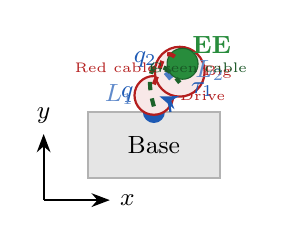
\begin{tikzpicture}[
    scale=1.4,
    >=Stealth,
    link/.style={line width=3pt, draw=drakeblue!80},
    joint/.style={circle, fill=drakeblue, inner sep=0, minimum size=8pt},
    pulley/.style={circle, draw=darkred, thick, minimum size=14pt, fill=darkred!10},
    cable/.style={line width=1.5pt, darkred},
    dim/.style={|<->|, thin, gray},
]
    % Base
    \filldraw[fill=gray!20, draw=gray!60, thick] (-0.6,-0.3) rectangle (0.6,0.3);
    \node at (0,0) {\small Base};

    % Joint 1
    \node[joint] (J1) at (0, 0.3) {};
    \node[above left, font=\small\bfseries, drakeblue] at (J1) {$q_1$};

    % Link 1
    \coordinate (L1end) at ({0.335*cos(70)}, {0.3 + 0.335*sin(70)});
    \draw[link] (J1.center) -- (L1end);
    \node[left, font=\small, text=drakeblue!70] at ($(J1.center)!0.5!(L1end) + (-0.15,0)$) {$L_1$};

    % Drive pulley (at J1)
    \node[pulley] at (0, 0.45) {};
    \node[right, font=\tiny, darkred] at (0.15, 0.45) {Drive};

    % Joint 2
    \node[joint] (J2) at (L1end) {};
    \node[above left, font=\small\bfseries, drakeblue] at (J2) {$q_2$};

    % Big pulley (at J2)
    \node[pulley, minimum size=18pt] at ($(L1end) + (0.12, 0.05)$) {};
    \node[right, font=\tiny, darkred] at ($(L1end) + (0.25, 0.05)$) {Big};

    % Link 2
    \coordinate (L2end) at ({0.335*cos(70) + 0.19*cos(40)}, {0.3 + 0.335*sin(70) + 0.19*sin(40)});
    \draw[link] (J2.center) -- (L2end);
    \node[right, font=\small, text=drakeblue!70] at ($(J2.center)!0.5!(L2end) + (0.1,0)$) {$L_2$};

    % EE
    \filldraw[fill=drakegreen, draw=drakegreen!70!black] (L2end) circle (4pt);
    \node[above right, font=\small\bfseries, drakegreen] at (L2end) {EE};

    % Cable routing (simplified)
    \draw[cable, dashed] (0, 0.55) .. controls (0.1, 0.8) and (0.08, 0.9) .. ($(L1end) + (0.12, 0.15)$);
    \draw[cable, dashed, drakegreen!70!black] (0, 0.35) .. controls (-0.1, 0.7) and (0.02, 0.85) .. ($(L1end) + (0.12, -0.05)$);
    \node[font=\tiny, darkred] at (-0.35, 0.7) {Red cable};
    \node[font=\tiny, drakegreen!60!black] at (0.4, 0.7) {Green cable};

    % Coordinate frame
    \draw[->, thick] (-1.0, -0.5) -- (-0.4, -0.5) node[right, font=\small] {$x$};
    \draw[->, thick] (-1.0, -0.5) -- (-1.0, 0.1) node[above, font=\small] {$y$};

    % Torque labels
    \draw[->, thick, drakeblue] (0.15, 0.3) arc[start angle=0, end angle=70, radius=0.15];
    \node[right, font=\small, drakeblue] at (0.25, 0.5) {$\tau_1$};

\end{tikzpicture}
\caption{2R cable-driven manipulator. Joint~1 is direct-drive; Joint~2 uses a cable routed through drive, idler, and big pulleys.}
\label{fig:robot_schematic}
\end{figure}

\subsection{CupManipulatorTendon --- Configuration Class}

The robot is represented by a frozen dataclass that stores all physical parameters, URDF paths, and joint configurations.  The class \texttt{CupManipulatorTendon} (in \texttt{robots/cup\_manipulator\_tendon.py}) wraps this config and provides Drake-facing methods:

\begin{lstlisting}[caption={Key constants and methods of \texttt{CupManipulatorTendon}.}]
class CupManipulatorTendon(RobotBase):
    # --- Joint names (matches URDF parse order) ---
    JT1_NAME  = "link1_base"      # q1: direct-drive
    JT2_NAME  = "link2_link1"     # q2: cable-driven
    ACT1_NAME = "tau_link1_base"
    ACT2_NAME = "tau_link2_link1"

    # --- End-effector frame offset on link2 ---
    EE_XYZ_LINK2 = [0.19, 0.0, 0.0515]   # [m]
    EE_FRAME_NAME = "tendon_ee"

    # --- Pulley parameters (HTD 5M 60T belt) ---
    PULLEY_RADIUS = 60 * 0.005 / (2 * np.pi)  # ~0.04775 m

    # Key methods:
    def load_urdf_to_plant(self, plant, parser):  ...
    def weld_base_to_world(self, plant, pos, orient):  ...
    def add_end_effector_frame(self, plant):  ...
    def add_joint_actuators(self, plant):  ...
    def get_state_from_plant(self, plant, ctx):  # [q1,q2,dq1,dq2]
    def compute_ik_analytical(self, plant, target_xy, q_seed):  ...
    def init_cable_rig(self, urdf_path, assets_dir):  ...
\end{lstlisting}

\begin{warnbox}
\textbf{Drake joint ordering caveat.}  Drake's \texttt{GetJointIndices()} returns joints in URDF parse order.  For the cable manipulator URDF this is \texttt{[link2\_link1, link1\_base]} = $[q_2, q_1]$, \emph{not} $[q_1, q_2]$.  The \texttt{get\_state\_from\_plant()} and \texttt{set\_state\_in\_plant()} helpers re-map to user order $[q_1, q_2]$ automatically.
\end{warnbox}

\subsection{CupManipulatorIK --- Inverse Kinematics Helper}

The \texttt{CupManipulatorIK} class (inner member \texttt{self.ik} of the manipulator) provides all kinematic queries:

\begin{lstlisting}[caption={IK helper methods.}]
class CupManipulatorIK:
    def get_link_lengths(self, plant) -> Tuple[float, float]:
        """Extract (L1, L2) from FK at q=0."""
        # L1 = |J1_origin - J2_origin| in XY plane
        # L2 = |J2_origin - EE_frame|   in XY plane

    def analytical(self, plant, target_xy, q_seed):
        """Closed-form 2R IK: returns (q_best, success)."""
        return self._solve_2r_core(L1, L2, target_xy, q_seed)

    def jacobian(self, plant, context) -> np.ndarray:
        """Drake automatic Jacobian via CalcJacobianTranslationalVelocity."""
        # Returns J in R^{2x2}: dp_EE = J(q) * dq

    def jacobian_analytical(self, plant, context) -> np.ndarray:
        """Closed-form planar Jacobian (no Drake call)."""
        # J = [[-L1*s1 - L2*s12, -L2*s12],
        #      [ L1*c1 + L2*c12,  L2*c12]]

    def velocity(self, plant, context, ee_vel, damping=1e-4):
        """Pseudo-inverse velocity IK: dq = pinv(J) @ ee_vel."""
\end{lstlisting}

\begin{codemath}
Link lengths are extracted once at construction time via forward kinematics at $\bq = \bm{0}$:
\[
    L_1 = \|\bm{p}_{J2} - \bm{p}_{J1}\|_{xy}, \qquad
    L_2 = \|\bm{p}_{\mathrm{EE}} - \bm{p}_{J2}\|_{xy}
\]
The \texttt{jacobian()} method uses Drake's articulated-body Jacobian (exact for the URDF model), while \texttt{jacobian\_analytical()} computes the planar $2\times 2$ matrix directly.  Both produce identical results for planar motion.
\end{codemath}


% ============================================================================
\section{Dynamics --- Manipulator Equation of Motion}
\label{sec:dynamics}
% ============================================================================

\subsection{Standard Manipulator Dynamics}

The equations of motion for a rigid-body manipulator are:

\begin{equation}
\boxed{
\bM(\bq)\,\bddq + \bm{C}(\bq, \bdq)\,\bdq + \bm{g}(\bq) = \btau
}
\label{eq:eom}
\end{equation}

where:
\begin{itemize}[leftmargin=2em]
    \item $\bq = [q_1, q_2]^\top$ --- joint positions [rad]
    \item $\bdq = [\dot q_1, \dot q_2]^\top$ --- joint velocities [rad/s]
    \item $\bM(\bq) \in \mathbb{R}^{2\times 2}$ --- symmetric positive-definite \textbf{mass (inertia) matrix}
    \item $\bm{C}(\bq, \bdq)\,\bdq \in \mathbb{R}^2$ --- \textbf{Coriolis and centrifugal} terms
    \item $\bm{g}(\bq) \in \mathbb{R}^2$ --- \textbf{gravitational} torques
    \item $\btau = [\tau_1, \tau_2]^\top$ --- applied joint torques [Nm]
\end{itemize}

We define the \textbf{bias vector} for compactness:
\begin{equation}
\bh(\bq, \bdq) \triangleq \bm{C}(\bq, \bdq)\,\bdq + \bm{g}(\bq)
\label{eq:bias}
\end{equation}

so that \eqref{eq:eom} becomes $\bM(\bq)\,\bddq + \bh(\bq, \bdq) = \btau$.

\subsection{2R Planar Arm --- Analytical Mass Matrix}

For a planar 2R arm with link lengths $L_1, L_2$, link masses $m_1, m_2$, and link inertias $I_1, I_2$:

\begin{equation}
\bM(\bq) = \begin{bmatrix}
    m_{11} & m_{12} \\
    m_{21} & m_{22}
\end{bmatrix}
\end{equation}

where:
\begin{align}
    m_{11} &= I_1 + I_2 + m_1 r_1^2 + m_2(L_1^2 + r_2^2 + 2L_1 r_2 \cos q_2) \\
    m_{12} = m_{21} &= I_2 + m_2(r_2^2 + L_1 r_2 \cos q_2) \\
    m_{22} &= I_2 + m_2 r_2^2
    \label{eq:mass_2r}
\end{align}

where $r_1, r_2$ are the distances from each joint to the respective link's center of mass.

\begin{warnbox}
In \textbf{PyDrake}, the mass matrix $\bM(\bq)$ is computed automatically by the MultibodyPlant via \texttt{plant.CalcMassMatrix(context)}. This uses the full URDF inertia tensors, including off-diagonal terms and 3D contributions projected onto the 2D plane --- which is more accurate than the analytical formula above.
\end{warnbox}

% ============================================================================
\section{Forward Kinematics and Jacobian}
\label{sec:fk_jac}
% ============================================================================

\subsection{Forward Kinematics}

The end-effector position in the world frame for the horizontal SCARA-like configuration:

\begin{equation}
\boxed{
\bm{p}_{\mathrm{EE}} = \begin{bmatrix}
    L_1 \cos q_1 + L_2 \cos(q_1 + q_2) \\
    L_1 \sin q_1 + L_2 \sin(q_1 + q_2)
\end{bmatrix}
}
\label{eq:fk}
\end{equation}

\subsection{Analytical Jacobian}

The Jacobian mapping joint velocities to EE velocities is:

\begin{equation}
\bJ(\bq) = \frac{\partial \bm{p}_{\mathrm{EE}}}{\partial \bq}
= \begin{bmatrix}
    -L_1 \sin q_1 - L_2 \sin(q_1 + q_2) & -L_2 \sin(q_1 + q_2) \\
     L_1 \cos q_1 + L_2 \cos(q_1 + q_2)  &  L_2 \cos(q_1 + q_2)
\end{bmatrix}
\label{eq:jacobian}
\end{equation}

so that $\dot{\bm{p}}_{\mathrm{EE}} = \bJ(\bq)\,\bdq$.

Denoting $s_1 = \sin q_1$, $c_1 = \cos q_1$, $s_{12} = \sin(q_1 + q_2)$, $c_{12} = \cos(q_1 + q_2)$:

\begin{equation}
\bJ = \begin{bmatrix}
    -L_1 s_1 - L_2 s_{12} & -L_2 s_{12} \\
     L_1 c_1 + L_2 c_{12}  &  L_2 c_{12}
\end{bmatrix}
\end{equation}

\begin{lstlisting}[caption={Analytical Jacobian --- \texttt{rl/computed\_torque\_controller.py}}]
# Analytical Jacobian at q_des
q1d, q2d = q_des
s1  = np.sin(q1d);   c1  = np.cos(q1d)
s12 = np.sin(q1d + q2d);  c12 = np.cos(q1d + q2d)
J = np.array([
    [-L1 * s1 - L2 * s12, -L2 * s12],
    [ L1 * c1 + L2 * c12,  L2 * c12],
])
\end{lstlisting}

\begin{codemath}
The code builds the $2\times 2$ Jacobian matrix from \eqref{eq:jacobian} using compact trigonometric notation. The pseudo-inverse $\bJ^{+} = \bJ^{-1}$ (since $\bJ$ is square and non-singular away from singularities) is then used to map Cartesian references to joint space:
\[
    \bdq_{\mathrm{ref}} = \bJ^{-1}\,\dot{\bm{x}}_{\mathrm{ref}}, \qquad
    \bddq_{\mathrm{ref}} \approx \bJ^{-1}\,\ddot{\bm{x}}_{\mathrm{ref}}
\]
where the $\dot{\bJ}\,\bdq$ bias term is dropped (order $O(\dot q^2)$, small for slow trajectories).
\end{codemath}

\subsection{Inverse Kinematics --- 2R Closed-Form Solution}

For a target $\bm{p}^* = [x^*, y^*]^\top$, the analytical IK solution is:

\begin{align}
    \cos q_2 &= \frac{x^{*2} + y^{*2} - L_1^2 - L_2^2}{2\,L_1\,L_2} \label{eq:ik_cosq2}\\
    q_2 &= \pm\arccos(\cos q_2) \qquad \text{(elbow up/down)} \label{eq:ik_q2}\\
    q_1 &= \operatorname{atan2}(y^*, x^*) - \operatorname{atan2}(L_2 \sin q_2,\; L_1 + L_2 \cos q_2) \label{eq:ik_q1}
\end{align}

Both elbow solutions are evaluated and the one \emph{closest to the seed} $\bq_{\mathrm{seed}}$ is returned:

\begin{lstlisting}[caption={2R IK solver --- \texttt{robots/cup\_manipulator\_tendon.py}}]
def _solve_2r_core(L1, L2, target_xy, q_seed, q2_limit):
    x_t, y_t = target_xy
    cos_q2 = (x_t**2 + y_t**2 - L1**2 - L2**2) / (2 * L1 * L2)
    cos_q2 = np.clip(cos_q2, -1.0, 1.0)
    candidates = []
    for sign in (+1, -1):
        q2 = sign * np.arccos(cos_q2)
        q1 = np.arctan2(y_t, x_t) - np.arctan2(
            L2 * np.sin(q2), L1 + L2 * np.cos(q2))
        candidates.append(np.array([q1, q2]))
    # Pick solution closest to seed
    best = min(candidates, key=lambda c: np.sum((c - q_seed)**2))
    return best, True
\end{lstlisting}

\begin{codemath}
Equations \eqref{eq:ik_cosq2}--\eqref{eq:ik_q1} are the standard closed-form inverse kinematics for a 2R planar arm. The seed-selection strategy ensures continuity along a trajectory:
\[
    \bq^* = \arg\min_{\bq \in \{\bq^+, \bq^-\}} \|\bq - \bq_{\mathrm{seed}}\|^2
\]
\end{codemath}

% ============================================================================
\section{Computed-Torque Control Law}
\label{sec:ct_law}
% ============================================================================

\subsection{Theory: Feedback Linearization}

The \textbf{computed-torque} (CT) controller achieves \emph{feedback linearization} of the nonlinear manipulator dynamics. Given a desired joint-space acceleration $\bm{a}_{\mathrm{des}}$, the control law cancels the nonlinear terms exactly:

\begin{equation}
\boxed{
\btau = \bM(\bq)\,\bm{a}_{\mathrm{des}} + \bh(\bq, \bdq)
}
\label{eq:ct_law}
\end{equation}

Substituting \eqref{eq:ct_law} into the dynamics \eqref{eq:eom}:

\begin{align}
    \bM(\bq)\,\bddq + \bh(\bq, \bdq) &= \bM(\bq)\,\bm{a}_{\mathrm{des}} + \bh(\bq, \bdq) \\
    \bM(\bq)\,\bddq &= \bM(\bq)\,\bm{a}_{\mathrm{des}} \\
    \bddq &= \bm{a}_{\mathrm{des}}
\end{align}

This is exact cancellation, reducing the controlled system to a \textbf{double integrator}:
\[
    \bddq = \bm{a}_{\mathrm{des}}
\]

\subsection{Desired Acceleration with Feedforward}

The desired acceleration includes both \textbf{feedforward (reference trajectory)} and \textbf{feedback (PD error correction)}:

\begin{equation}
\boxed{
\bm{a}_{\mathrm{des}} = \bddq_{\mathrm{ref}} + K_p\,(\bq_{\mathrm{des}} - \bq) + K_d\,(\bdq_{\mathrm{ref}} - \bdq)
}
\label{eq:a_des}
\end{equation}

\noindent where:
\begin{itemize}[leftmargin=2em]
    \item $\bq_{\mathrm{des}}$ --- desired joint position from IK
    \item $\bdq_{\mathrm{ref}}$ --- desired joint velocity: $\bdq_{\mathrm{ref}} = \bJ^{-1}\,\dot{\bm{x}}_{\mathrm{ref}}$
    \item $\bddq_{\mathrm{ref}}$ --- desired joint acceleration: $\bddq_{\mathrm{ref}} \approx \bJ^{-1}\,\ddot{\bm{x}}_{\mathrm{ref}}$
    \item $K_p, K_d$ --- scalar proportional and derivative gains
\end{itemize}

\subsection{Closed-Loop Error Dynamics}

Define the tracking error $\bm{e} = \bq - \bq_{\mathrm{des}}$. Since $\bddq = \bm{a}_{\mathrm{des}}$:

\begin{equation}
    \ddot{\bm{e}} + K_d\,\dot{\bm{e}} + K_p\,\bm{e} = \bm{0}
\end{equation}

This is a decoupled \textbf{second-order linear ODE} for each joint. The characteristic equation is:
\begin{equation}
    s^2 + K_d\,s + K_p = 0
\end{equation}

with natural frequency and damping ratio:
\begin{equation}
\boxed{
    \omega_n = \sqrt{K_p}, \qquad \zeta = \frac{K_d}{2\,\omega_n} = \frac{K_d}{2\sqrt{K_p}}
}
\label{eq:gains}
\end{equation}

\begin{resultbox}
For $K_p = 400$, $K_d = 40$: $\omega_n = 20$\,rad/s, $\zeta = 1.0$ \textbf{(critically damped)}. The error decays as $e(t) \sim (c_1 + c_2 t)\,e^{-\omega_n t}$ with time constant $T = 1/\omega_n = 50$\,ms.
\end{resultbox}

\subsection{Full Controller Code}

\begin{lstlisting}[caption={Computed-torque law --- \texttt{rl/computed\_torque\_controller.py}}]
def compute(self, q, q_dot, q_des, q_dot_ref, q_ddot_ref, M, h):
    """
    a_des = q_ddot_ref + Kp*(q_des - q) + Kd*(q_dot_ref - q_dot)
    tau   = M(q) @ a_des + h(q, q_dot)
    """
    a_des = q_ddot_ref + self.Kp * (q_des - q) \
                       + self.Kd * (q_dot_ref - q_dot)
    tau_raw = M @ a_des + h

    # Cable tension decomposition for joint 2
    F_net = tau_raw[1] / self.r_p
    T_green = max(F_net, 0.0)    # retracting side
    T_red   = max(-F_net, 0.0)   # extending side
    tau2_cmd = (T_green - T_red) * self.r_p

    tau_clip = np.clip(
        np.array([tau_raw[0], tau2_cmd]),
        -self.tau_max, self.tau_max
    )
    return CTControllerOutput(tau_clip=tau_clip, tau_raw=tau_raw, ...)
\end{lstlisting}

\begin{codemath}
The controller implements equations \eqref{eq:ct_law} and \eqref{eq:a_des} in three steps:

\textbf{Step 1 --- PD + Feedforward acceleration:}
\[
    \bm{a}_{\mathrm{des}} = \bddq_{\mathrm{ref}} + K_p\,(\bq_{\mathrm{des}} - \bq) + K_d\,(\bdq_{\mathrm{ref}} - \bdq)
\]

\textbf{Step 2 --- Inverse dynamics:}
\[
    \btau_{\mathrm{raw}} = \bM(\bq)\,\bm{a}_{\mathrm{des}} + \bh(\bq, \bdq)
\]

\textbf{Step 3 --- Cable tension decomposition (joint~2):}
\[
    F_{\mathrm{net}} = \frac{\tau_2}{\rp}, \qquad
    T_{\mathrm{green}} = \max(F_{\mathrm{net}}, 0), \qquad
    T_{\mathrm{red}} = \max(-F_{\mathrm{net}}, 0)
\]
\[
    \tau_{2,\mathrm{cmd}} = (T_{\mathrm{green}} - T_{\mathrm{red}}) \cdot \rp
\]

Finally, the torque is clipped: $\btau_{\mathrm{clip}} = \mathrm{clip}(\btau, -\tau_{\max}, +\tau_{\max})$.
\end{codemath}


% ============================================================================
\section{Pure NumPy Controller Engine}
\label{sec:numpy_ct}
% ============================================================================

The engine-agnostic controller lives in \texttt{rl/computed\_torque\_controller.py}.  It contains \textbf{zero Drake imports}---only NumPy---so it can be shared between PyDrake and Isaac Sim.

\subsection{CTControllerOutput Dataclass}

\begin{lstlisting}[caption={Output bundle from each control cycle.}]
@dataclass
class CTControllerOutput:
    tau_clip: np.ndarray     # [2] clipped torques [Nm]
    tau_raw: np.ndarray      # [2] pre-saturation torques [Nm]
    T_green: float           # retracting cable tension [N]
    T_red: float             # extending cable tension [N]
    q_des: np.ndarray        # [2] desired joint positions [rad]
    a_des: np.ndarray        # [2] desired joint accelerations [rad/s^2]
\end{lstlisting}

\subsection{ComputedTorqueController Class}

\begin{lstlisting}[caption={Pure NumPy CT controller --- \texttt{rl/computed\_torque\_controller.py}}]
class ComputedTorqueController:
    def __init__(self, Kp=400.0, Kd=40.0, tau_max=10.0,
                 pulley_radius=0.04775):
        self.Kp = Kp
        self.Kd = Kd
        self.tau_max = tau_max
        self.pulley_radius = pulley_radius

    @property
    def omega_n(self): return np.sqrt(self.Kp)   # natural freq [rad/s]

    @property
    def zeta(self): return self.Kd / (2*self.omega_n)  # damping ratio

    def compute(self, q, q_dot, q_des, q_dot_ref, q_ddot_ref,
                M, h) -> CTControllerOutput:
        # --- PD + feedforward ---
        a_des = (q_ddot_ref
                 + self.Kp * (q_des - q)
                 + self.Kd * (q_dot_ref - q_dot))

        # --- Inverse dynamics ---
        tau_raw = M @ a_des + h

        # --- Cable tension decomposition (joint 2) ---
        F_net = tau_raw[1] / self.pulley_radius
        T_green = max(F_net, 0.0)
        T_red   = max(-F_net, 0.0)

        # --- Saturation ---
        tau_clip = np.clip(tau_raw, -self.tau_max, self.tau_max)

        return CTControllerOutput(
            tau_clip=tau_clip, tau_raw=tau_raw,
            T_green=T_green, T_red=T_red,
            q_des=q_des, a_des=a_des)
\end{lstlisting}

\begin{codemath}
The \texttt{compute()} method executes the full CT pipeline in five lines:
\begin{enumerate}
    \item \textbf{PD + Feedforward}: $\bm{a}_{\mathrm{des}} = \bddq_{\mathrm{ref}} + K_p(\bq_{\mathrm{des}} - \bq) + K_d(\bdq_{\mathrm{ref}} - \bdq)$
    \item \textbf{Inverse Dynamics}: $\btau_{\mathrm{raw}} = \bM(\bq)\,\bm{a}_{\mathrm{des}} + \bh(\bq, \bdq)$
    \item \textbf{Cable Decomposition}: $F_{\mathrm{net}} = \tau_2 / r_p$, then $T_g = \max(F,0)$, $T_r = \max(-F,0)$
    \item \textbf{Saturation}: $\btau_{\mathrm{clip}} = \mathrm{clip}(\btau, -\tau_{\max}, +\tau_{\max})$
\end{enumerate}
The cable tension decomposition ensures the physical constraint that cables can only \emph{pull} (unidirectional force).
\end{codemath}

\subsection{EE-to-Joint Reference Conversion}

The helper function \texttt{ik\_to\_joint\_space\_references()} maps end-effector references to joint space:

\begin{lstlisting}[caption={EE-to-joint conversion --- \texttt{rl/computed\_torque\_controller.py}}]
def ik_to_joint_space_references(
    ee_pos_ref, ee_vel_ref, ee_acc_ref,   # EE targets [m, m/s, m/s^2]
    L1, L2,                                # link lengths [m]
    q_seed,                                # warm-start for IK [rad]
    solve_ik_fn,                           # callback for 2R IK solver
) -> Tuple[np.ndarray, np.ndarray, np.ndarray, bool]:
    # 1. Position IK
    q_des, ok = solve_ik_fn(L1, L2, ee_pos_ref, q_seed)

    # 2. Analytical Jacobian at q_des
    s1, c1 = np.sin(q_des[0]), np.cos(q_des[0])
    s12 = np.sin(q_des[0] + q_des[1])
    c12 = np.cos(q_des[0] + q_des[1])
    J = np.array([[-L1*s1 - L2*s12, -L2*s12],
                  [ L1*c1 + L2*c12,  L2*c12]])

    # 3. Pseudo-inverse mapping
    J_inv = np.linalg.pinv(J)
    q_dot_ref  = J_inv @ ee_vel_ref
    q_ddot_ref = J_inv @ ee_acc_ref   # ignores Jdot*qdot bias

    return q_des, q_dot_ref, q_ddot_ref, ok
\end{lstlisting}

\begin{codemath}
The velocity/acceleration mapping uses the first-order approximation:
\[
    \bdq_{\mathrm{ref}} = \bJ^{-1}\,\dot{\bm{x}}_{\mathrm{ref}}, \qquad
    \bddq_{\mathrm{ref}} \approx \bJ^{-1}\,\ddot{\bm{x}}_{\mathrm{ref}}
\]

\begin{warnbox}
The acceleration mapping omits the $\dot{\bJ}\bdq$ term.  For slow trajectories this is negligible, but for high-speed motions the missing Coriolis coupling introduces a small feedforward error.  The PD gains absorb this error in practice ($<1$\,mm tracking at 0.08\,m/s).
\end{warnbox}
\end{codemath}


% ============================================================================
\section{PyDrake Architecture --- Two-Plant Diagram Pattern}
\label{sec:architecture}
% ============================================================================

\subsection{Drake Diagram Overview}

The PyDrake implementation uses Drake's \textbf{Systems Framework} with a \texttt{DiagramBuilder} to wire signal connections between \texttt{LeafSystem} blocks:

\begin{archbox}{Signal-Flow Diagram}
\begin{center}
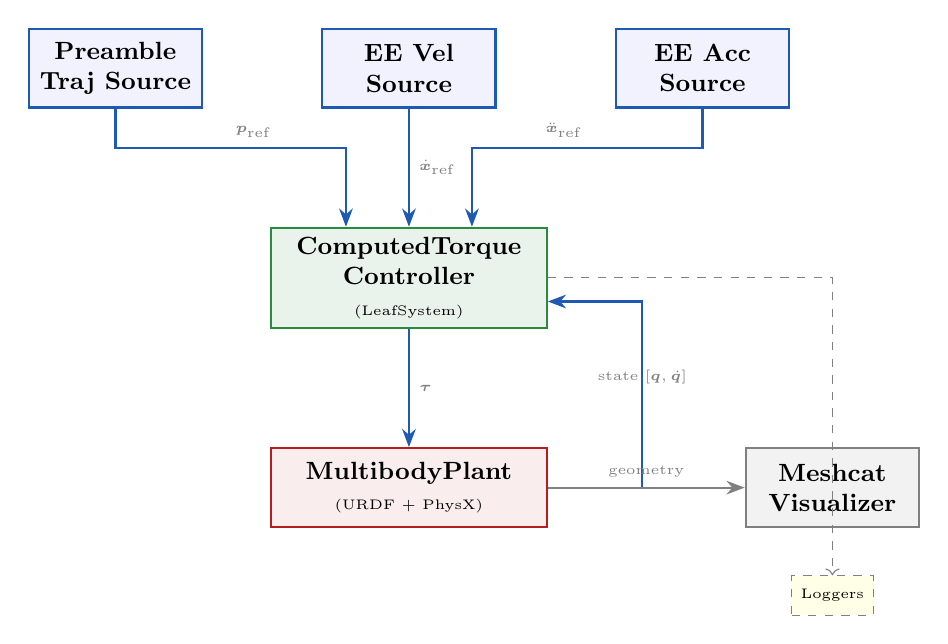
\begin{tikzpicture}[
    node distance=1.2cm and 1.8cm,
    block/.style={rectangle, draw=drakeblue, thick, fill=blue!5,
                  minimum height=1.0cm, minimum width=2.2cm, align=center,
                  font=\small},
    port/.style={font=\tiny, text=gray},
    arr/.style={-Stealth, thick, drakeblue},
]
    % Blocks
    \node[block] (traj) {\textbf{Preamble}\\\textbf{Traj Source}};
    \node[block, right=1.5cm of traj] (vel) {\textbf{EE Vel}\\\textbf{Source}};
    \node[block, right=1.5cm of vel] (acc) {\textbf{EE Acc}\\\textbf{Source}};

    \node[block, below=1.5cm of vel, minimum width=3.5cm, fill=drakegreen!10, draw=drakegreen] (ct) {\textbf{ComputedTorque}\\\textbf{Controller}\\{\tiny (LeafSystem)}};

    \node[block, below=1.5cm of ct, minimum width=3.5cm, fill=darkred!8, draw=darkred] (plant) {\textbf{MultibodyPlant}\\{\tiny (URDF + PhysX)}};

    \node[block, right=2.5cm of plant, fill=gray!10, draw=gray] (meshcat) {\textbf{Meshcat}\\\textbf{Visualizer}};

    % Connections
    \draw[arr] (traj.south) -- ++(0,-0.5) -| ([xshift=-0.8cm]ct.north) node[pos=0.3, above, port] {$\bm{p}_{\mathrm{ref}}$};
    \draw[arr] (vel.south) -- (ct.north) node[pos=0.5, right, port] {$\dot{\bm{x}}_{\mathrm{ref}}$};
    \draw[arr] (acc.south) -- ++(0,-0.5) -| ([xshift=0.8cm]ct.north) node[pos=0.3, above, port] {$\ddot{\bm{x}}_{\mathrm{ref}}$};

    \draw[arr] (ct.south) -- (plant.north) node[pos=0.5, right, port] {$\btau$};

    \draw[arr] (plant.east) -- ++(1.2,0) |- ([yshift=-0.3cm]ct.east) node[pos=0.25, above, port] {state $[\bq, \bdq]$};

    \draw[arr, gray] (plant.east) -- (meshcat.west) node[pos=0.5, above, port] {geometry};

    % Loggers (small)
    \node[rectangle, draw=gray, dashed, fill=yellow!10, minimum height=0.5cm, font=\tiny, below=0.6cm of meshcat] (log) {Loggers};
    \draw[->, dashed, gray] (ct.east) -| (log.north);
\end{tikzpicture}
\end{center}
\end{archbox}

\subsection{ComputedTorqueController --- Drake LeafSystem}

In the PyDrake version, the controller is a \texttt{LeafSystem} with four input ports and four output ports:

\begin{table}[h]
\centering
\caption{Controller I/O ports.}
\begin{tabular}{lll}
\toprule
\textbf{Direction} & \textbf{Port Name} & \textbf{Size / Description} \\
\midrule
Input  & \texttt{desired\_ee\_pos} & 2 --- $[x_{\mathrm{ref}}, y_{\mathrm{ref}}]$ \\
Input  & \texttt{ee\_vel\_ref}     & 2 --- $[\dot x_{\mathrm{ref}}, \dot y_{\mathrm{ref}}]$ \\
Input  & \texttt{ee\_acc\_ref}     & 2 --- $[\ddot x_{\mathrm{ref}}, \ddot y_{\mathrm{ref}}]$ \\
Input  & \texttt{plant\_state}     & $n_q + n_v$ --- full state vector \\
\midrule
Output & \texttt{actuation}        & 2 --- clipped $[\tau_1, \tau_2]$ \\
Output & \texttt{joint\_positions}  & 2 --- desired $[q_{1,\mathrm{des}}, q_{2,\mathrm{des}}]$ \\
Output & \texttt{torques\_raw}      & 2 --- pre-clip $[\tau_{1,\mathrm{raw}}, \tau_{2,\mathrm{raw}}]$ \\
Output & \texttt{cable\_tensions}   & 2 --- $[T_{\mathrm{green}}, T_{\mathrm{red}}]$ \\
\bottomrule
\end{tabular}
\end{table}

The key computation happens in the output callback, which:
\begin{enumerate}[leftmargin=2em]
    \item Reads the current state $(\bq, \bdq)$ from the plant state port
    \item Solves IK: $\bm{p}_{\mathrm{ref}} \to \bq_{\mathrm{des}}$
    \item Computes $\bdq_{\mathrm{ref}} = \bJ^{-1}\,\dot{\bm{x}}_{\mathrm{ref}}$ and $\bddq_{\mathrm{ref}} \approx \bJ^{-1}\,\ddot{\bm{x}}_{\mathrm{ref}}$
    \item Evaluates $\btau = \bM\,\bm{a}_{\mathrm{des}} + \bh$ using Drake's \texttt{CalcMassMatrix} and \texttt{CalcBiasTerm}
    \item Clips and returns the torque
\end{enumerate}

\begin{lstlisting}[caption={Drake LeafSystem-based CT controller (simplified) --- \texttt{robots/cup\_manipulator\_tendon.py}}]
class ComputedTorqueController(LeafSystem):
    def __init__(self, plant, manipulator, Kp, Kd, tau_max):
        super().__init__()
        self._plant = plant          # physics MultibodyPlant
        self._manip = manipulator    # CupManipulatorTendon config
        self._Kp = Kp;  self._Kd = Kd;  self._tau_max = tau_max

        # Create internal plant context for dynamics queries
        self._ctrl_context = plant.CreateDefaultContext()

        # Declare I/O ports
        self.DeclareVectorInputPort("desired_ee_pos", 2)
        self.DeclareVectorInputPort("ee_vel_ref", 2)
        self.DeclareVectorInputPort("ee_acc_ref", 2)
        self.DeclareVectorInputPort("plant_state", plant.num_positions()
                                                   + plant.num_velocities())
        self.DeclareVectorOutputPort("actuation", 2, self._calc_torque)
        # ... additional output ports ...

    def _calc_torque(self, context, output):
        # 1. Read state
        state = self.get_input_port(3).Eval(context)
        self._plant.SetPositionsAndVelocities(self._ctrl_context, state)
        q = state[:nq];  q_dot = state[nq:]

        # 2. IK: EE ref -> joint ref
        ee_ref = self.get_input_port(0).Eval(context)
        q_des, ok = self._manip.ik.analytical(self._plant, ee_ref, q_seed)

        # 3. Jacobian -> joint velocity/acceleration refs
        J = self._manip.ik.jacobian_analytical(self._plant, self._ctrl_context)
        J_inv = np.linalg.pinv(J)
        q_dot_ref  = J_inv @ ee_vel_ref
        q_ddot_ref = J_inv @ ee_acc_ref

        # 4. Dynamics
        M = self._plant.CalcMassMatrix(self._ctrl_context)
        h = self._plant.CalcBiasTerm(self._ctrl_context)

        # 5. CT law
        a_des = q_ddot_ref + Kp*(q_des - q) + Kd*(q_dot_ref - q_dot)
        tau = M @ a_des + h
        output.SetFromVector(np.clip(tau, -tau_max, tau_max))
\end{lstlisting}

\begin{codemath}
The Drake \texttt{LeafSystem} executes the full CT pipeline every simulation step:
\begin{enumerate}
    \item \textbf{IK}: $\bm{p}_{\mathrm{ref}} \xrightarrow{\text{2R analytical}} \bq_{\mathrm{des}}$
    \item \textbf{Differential IK}: $\dot{\bm{x}}_{\mathrm{ref}} \xrightarrow{\bJ^{-1}} \bdq_{\mathrm{ref}}$, \quad $\ddot{\bm{x}}_{\mathrm{ref}} \xrightarrow{\bJ^{-1}} \bddq_{\mathrm{ref}}$
    \item \textbf{PD + FF}: $\bm{a}_{\mathrm{des}} = \bddq_{\mathrm{ref}} + K_p(\bq_{\mathrm{des}} - \bq) + K_d(\bdq_{\mathrm{ref}} - \bdq)$
    \item \textbf{Inverse Dynamics}: $\btau = \bM(\bq)\,\bm{a}_{\mathrm{des}} + \bh(\bq, \bdq)$
\end{enumerate}

Drake's \texttt{CalcMassMatrix} and \texttt{CalcBiasTerm} use the full articulated-body algorithm (Featherstone), which is exact for the URDF inertia model.
\end{codemath}


% ============================================================================
\section{Trajectory Generation}
\label{sec:trajectory}
% ============================================================================

\subsection{C$^2$ Cubic Spline Trajectories}

All trajectories use \textbf{periodic cubic splines} (via \texttt{scipy.CubicSpline} with \texttt{bc\_type='periodic'}) to ensure continuous position, velocity, and acceleration at the loop boundary:

\begin{equation}
    \bm{p}(t), \; \dot{\bm{p}}(t), \; \ddot{\bm{p}}(t) \in C^2 \qquad \text{for all } t
\end{equation}

\subsection{Rectangle Trajectory with Velocity Profiling}

The rectangle trajectory uses \textbf{non-uniform time stamps} to create slow-fast-slow velocity profiles:

\begin{enumerate}[leftmargin=2em]
    \item Distribute $N$ waypoints uniformly in \textbf{arc length} along the rectangle perimeter $P = 2(W + H)$
    \item At each waypoint, compute the \textbf{desired speed} using a smoothstep blend between corner speed $v_{\mathrm{corner}}$ and straight speed $v_{\mathrm{max}}$:
    \begin{equation}
        v(s) = v_{\mathrm{corner}} + (v_{\mathrm{max}} - v_{\mathrm{corner}}) \cdot h\!\left(\frac{d(s)}{d_{\mathrm{blend}}}\right)
    \end{equation}
    where $d(s)$ is the distance to the nearest corner and $h(t) = t^2(3 - 2t)$ is the Hermite smoothstep.
    \item Convert arc-length spacing to \textbf{time stamps} via $\Delta t_i = \Delta s / \bar{v}_i$ and rescale to the desired lap duration.
\end{enumerate}

\begin{lstlisting}[caption={Velocity profiling for rectangle corners --- \texttt{rl/trajectory.py}}]
def speed(s):
    t = np.clip(dist_corner(s) / d_blend, 0.0, 1.0)
    return v_corner + (v_max - v_corner) * t * t * (3.0 - 2.0 * t)

# Arc-length uniform, time non-uniform
ds = P / N
for i in range(N):
    t_raw[i+1] = t_raw[i] + ds / (0.5 * (speeds[i] + speeds[i+1]))
t_wp = t_raw * (lap_duration / t_raw[-1])
\end{lstlisting}

\begin{codemath}
The key idea: \textbf{uniform arc-length $\to$ non-uniform time}. The time between waypoints $i$ and $i+1$ is:
\[
    \Delta t_i = \frac{\Delta s}{\bar{v}_i}, \qquad \bar{v}_i = \frac{v(s_i) + v(s_{i+1})}{2}
\]
where $\Delta s = P/N$ is the constant arc-length spacing. The raw times are then rescaled to match the desired lap duration $T_{\mathrm{lap}}$:
\[
    t_i^{\mathrm{scaled}} = t_i^{\mathrm{raw}} \cdot \frac{T_{\mathrm{lap}}}{t_N^{\mathrm{raw}}}
\]
\end{codemath}

\subsection{Circle and Line Trajectories}

In addition to the rectangle, two simpler trajectory shapes are available:

\begin{lstlisting}[caption={Circle and line trajectory constructors --- \texttt{rl/trajectory.py}}]
class CircleTrajectory:
    def __init__(self, cx, cy, radius, N=60, lap_duration=10.0):
        theta = np.linspace(0, 2*np.pi, N+1)      # uniform angular spacing
        x = cx + radius * np.cos(theta)
        y = cy + radius * np.sin(theta)
        t = np.linspace(0, lap_duration, N+1)      # uniform time
        self._spline = LoopingCubicTrajectory(t, np.c_[x, y], lap_duration)

class LineTrajectory:
    def __init__(self, cx, cy, radius, N=60, lap_duration=10.0):
        # Forward + reverse + closure (back-and-forth on a line segment)
        x_fwd = np.linspace(cx - radius, cx + radius, N//2)
        x_rev = np.flip(x_fwd)
        x = np.concatenate([x_fwd, x_rev, [x_fwd[0]]])   # close the loop
        y = np.full_like(x, cy)
        # ...
\end{lstlisting}

All trajectory classes share the same interface: \texttt{eval\_position(t)}, \texttt{eval\_velocity(t)}, \texttt{eval\_acceleration(t)}.  This allows the simulation to be trajectory-agnostic.

\subsection{Move-to-Start Preamble}

Before trajectory tracking begins, the arm moves from its initial pose to the first waypoint using a \textbf{cubic Hermite spline}:

\begin{equation}
    \bm{p}(t) = \bm{H}(t/T_{\mathrm{move}}) \quad \text{with} \quad
    \bm{p}(0) = \bm{p}_{\mathrm{start}},\;
    \dot{\bm{p}}(0) = \bm{0},\;
    \bm{p}(T) = \bm{p}_{\mathrm{end}},\;
    \dot{\bm{p}}(T) = \dot{\bm{p}}_{\mathrm{traj}}(0)
\end{equation}

This ensures:
\begin{itemize}[leftmargin=2em]
    \item \textbf{Zero initial velocity} (robot starts from rest)
    \item \textbf{$C^1$ continuity} at the handoff to the main trajectory (velocity-matched)
\end{itemize}

\begin{lstlisting}[caption={Preamble source switches between move and main --- \texttt{rl/trajectory.py}}]
class PreambleTrajectorySource:
    def eval_position(self, t):
        if self._move is not None and t < self.move_duration:
            return self._move.eval_position(t)
        t_main = max(0.0, t - self.move_duration)
        return self._main.eval_position(t_main)
\end{lstlisting}


% ============================================================================
\section{Cable Routing and Tension Decomposition}
\label{sec:cables}
% ============================================================================

\subsection{Belt-Pulley Kinematics}

Joint~2 is actuated through a cable (HTD\,5M timing belt) routed as:

\begin{center}
\textbf{Motor} $\xrightarrow{\text{belt}}$ \textbf{Drive Pulley} $\to$ \textbf{Idler (L/R)} $\to$ \textbf{Big Pulley} $\to$ \textbf{Cable Endpoint}
\end{center}

The relationship between cable force and joint torque:

\begin{equation}
    \tau_2 = F_{\mathrm{net}} \cdot \rp = (T_{\mathrm{green}} - T_{\mathrm{red}}) \cdot \rp
\end{equation}

where $T_{\mathrm{green}} \geq 0$ is the tension on the retracting side (pulling) and $T_{\mathrm{red}} \geq 0$ is the tension on the extending side (releasing). Since cables can only pull:

\begin{equation}
    T_{\mathrm{green}} = \max\!\left(\frac{\tau_2}{\rp}, 0\right), \qquad
    T_{\mathrm{red}} = \max\!\left(-\frac{\tau_2}{\rp}, 0\right)
    \label{eq:tension_decomp}
\end{equation}

\subsection{Cable Visualization via DrakeCablePlant}

The cable geometry is computed by a headless Drake plant (\texttt{cable.py}):

\begin{lstlisting}[caption={Cable FK pipeline.}]
from cable import DrakeCablePlant

drake_cable = DrakeCablePlant(urdf_path, q1, q2)
drake_cable.update(q1_new, q2_new)       # sync joint angles
points = drake_cable.get_cable_world_points()  # [(route, pts), ...]
arcs   = drake_cable.get_wrap_arcs()            # pulley wrap arcs
\end{lstlisting}

The cable routing uses tangent-line geometry between pulleys:
\begin{itemize}[leftmargin=2em]
    \item \textbf{External tangent}: when cables wrap on the same side of two pulleys
    \item \textbf{Internal tangent}: when cables cross between pulleys
    \item Tangent points computed from 2D circle-to-circle geometry, then transformed to 3D world frame via FK
\end{itemize}

\subsection{Pulley Class Hierarchy}

All cable-routing primitives inherit from \texttt{PulleyBase} (defined in \texttt{cable.py}).  The hierarchy loads OBJ meshes via \texttt{trimesh} to auto-compute centroids and radii:

\begin{archbox}{Pulley Hierarchy}
\begin{center}
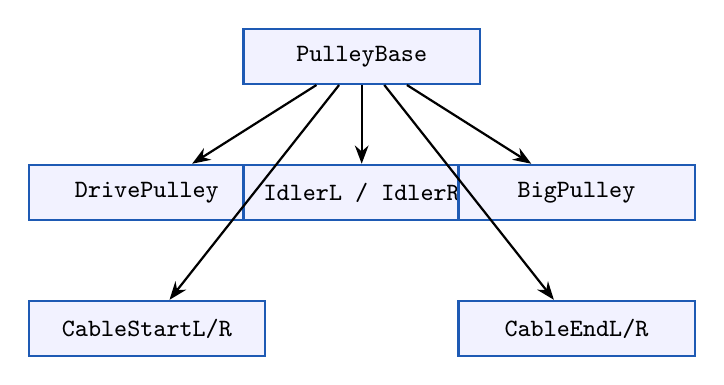
\begin{tikzpicture}[
    node distance=1cm and 1.5cm,
    cls/.style={rectangle, draw=drakeblue, thick, fill=blue!5,
                minimum height=0.7cm, minimum width=3cm, align=center, font=\small},
    arr/.style={-Stealth, thick},
]
    \node[cls] (base) {\texttt{PulleyBase}};
    \node[cls, below left=1cm and -0.3cm of base] (drive) {\texttt{DrivePulley}};
    \node[cls, below=1cm of base] (idler) {\texttt{IdlerL / IdlerR}};
    \node[cls, below right=1cm and -0.3cm of base] (big) {\texttt{BigPulley}};
    \node[cls, below=1cm of drive] (start) {\texttt{CableStartL/R}};
    \node[cls, below=1cm of big] (end) {\texttt{CableEndL/R}};

    \draw[arr] (base) -- (drive);
    \draw[arr] (base) -- (idler);
    \draw[arr] (base) -- (big);
    \draw[arr] (base) -- (start);
    \draw[arr] (base) -- (end);
\end{tikzpicture}
\end{center}
\end{archbox}

Each subclass specifies its OBJ mesh filename, URDF body name, and shaft direction.  The base class lazily computes:
\begin{itemize}[leftmargin=2em]
    \item \textbf{Centroid}: mesh geometric centre, rotated by URDF visual-origin RPY into body frame
    \item \textbf{Radius}: maximum perpendicular distance from centroid to shaft axis
\end{itemize}

\begin{lstlisting}[caption={PulleyBase mesh property computation --- \texttt{cable.py}}]
class PulleyBase:
    def _compute_centroid(self) -> np.ndarray:
        mesh = trimesh.load(os.path.join(self.assets_dir, self.obj_name))
        R = self._R_vis()   # rotation from URDF visual-origin RPY
        return R @ mesh.centroid + np.array(self.vis_xyz)

    def _compute_radius(self) -> float:
        mesh = trimesh.load(os.path.join(self.assets_dir, self.obj_name))
        R = self._R_vis()
        verts_body = (R @ mesh.vertices.T).T + np.array(self.vis_xyz)
        axis = self.shaft_axis_body
        # Max perpendicular distance from centroid to shaft axis
        return max(|v - centroid - proj(v-centroid, axis)| for v in verts_body)
\end{lstlisting}

\subsection{Tangent-Line Geometry}

The cable contact points between two pulleys are computed via \textbf{circle--circle tangent lines}.  Given two coplanar circles $(\bm{c}_1, r_1)$ and $(\bm{c}_2, r_2)$ separated by distance $D = \|\bm{c}_2 - \bm{c}_1\|$:

\paragraph{External tangent} (cables wrap same side):
\begin{align}
    \cos\alpha &= \frac{r_1 - r_2}{D}, \qquad \sin\alpha = \sqrt{1 - \cos^2\alpha} \nonumber \\
    \hat{\bm{n}} &= \cos\alpha\,\hat{\bm{d}} + s\,\sin\alpha\,\hat{\bm{d}}^\perp \quad (s = \pm 1) \nonumber \\
    \bm{T}_1 &= \bm{c}_1 + r_1\,\hat{\bm{n}}, \qquad \bm{T}_2 = \bm{c}_2 + r_2\,\hat{\bm{n}}
    \label{eq:ext_tangent}
\end{align}

\paragraph{Internal tangent} (cables cross between pulleys):
\begin{align}
    \cos\alpha &= \frac{r_1 + r_2}{D} \nonumber \\
    \bm{T}_1 &= \bm{c}_1 + r_1\,\hat{\bm{n}}, \qquad \bm{T}_2 = \bm{c}_2 - r_2\,\hat{\bm{n}}
    \label{eq:int_tangent}
\end{align}

The parameter $s \in \{+1, -1\}$ selects which of the two parallel tangent lines to use (upper vs.\ lower).  These 2D contact points are computed in the XY plane, with Z preserved from each pulley's centroid.

\subsection{CableRig --- Route Assembly}

The \texttt{CableRig} class aggregates all pulleys and cable anchors, defining the two tendon routes:

\begin{lstlisting}[caption={Cable route definitions --- \texttt{cable.py}}]
@dataclass
class CableRoute:
    segments: list             # [(waypoint_cfg, offset), ...]
    meshcat_path: str          # e.g., "/cable/green"
    meshcat_color: Rgba        # color for visualization
    label: str                 # "Green (Drive->IdlerR->Big->EndL)"

class CableRig:
    def __init__(self):
        # Green: Start_R -> Drive -> IdlerR -> BigPulley -> EndL
        self.cable_green = CableRoute(...)
        # Red:   Start_L -> Drive -> IdlerL -> BigPulley -> EndR
        self.cable_red = CableRoute(...)

    def compute_tangents(self, plant, plant_context, manipulator):
        """Update all inter-pulley tangent contact points via FK."""
        # 6 tangent pairs: Drive<->IdlerR, IdlerR<->Big, Big<->EndL
        #                   Drive<->IdlerL, IdlerL<->Big, Big<->EndR
        # Each uses tangent_in_world_frame() with appropriate branch/kind
\end{lstlisting}

\begin{codemath}
The \texttt{compute\_tangents()} method must be called whenever the joint configuration changes, because cross-frame tangent pairs (e.g., IdlerR on link1 $\leftrightarrow$ BigPulley on link2) are kinematically coupled via $q_2$.  Each call performs 6 pairs of FK + tangent computations.
\end{codemath}

\subsection{CableSpring --- Optional Compliance}

Optional helical springs at cable endpoints provide compliance and visual feedback:

\begin{lstlisting}[caption={Spring visualization --- \texttt{cable.py}}]
@dataclass
class CableSpring:
    stiffness: float = 100.0     # [N/m]
    rest_length: float = 0.002   # [m]
    n_coils: int = 6             # helical turns
    amplitude: float = 0.004    # helix radius [m]
    enabled: bool = True

def spring_zigzag_points(p_start, p_end, n_coils, amplitude):
    """Generate 3D helix for Meshcat visualization."""
    ax = (p_end - p_start) / np.linalg.norm(p_end - p_start)
    perp1, perp2 = orthonormal_frame(ax)
    # p(t) = p_start + ax*t + amplitude*(cos*perp1 + sin*perp2)
\end{lstlisting}


% ============================================================================
\section{Simulation --- Builder Pattern}
\label{sec:sim}
% ============================================================================

\subsection{ComputedTorqueSimulation Class Hierarchy}

\begin{archbox}{Class Hierarchy}
\begin{center}
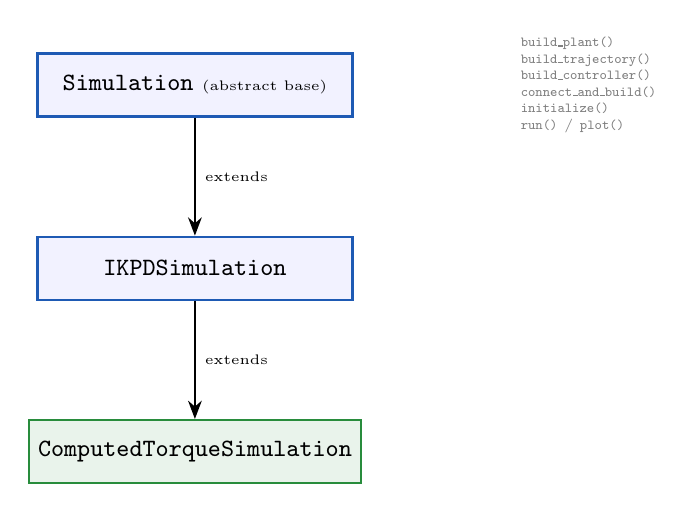
\begin{tikzpicture}[
    node distance=1.5cm,
    class/.style={rectangle, draw=drakeblue, thick, fill=blue!5,
                  minimum height=0.8cm, minimum width=4cm, align=center, font=\small},
    arr/.style={-Stealth, thick},
]
    \node[class] (sim) {\texttt{Simulation} {\tiny (abstract base)}};
    \node[class, below=of sim] (ikpd) {\texttt{IKPDSimulation}};
    \node[class, below=of ikpd, fill=drakegreen!10, draw=drakegreen] (ct) {\texttt{ComputedTorqueSimulation}};

    \draw[arr] (sim) -- (ikpd) node[midway, right, font=\tiny] {extends};
    \draw[arr] (ikpd) -- (ct) node[midway, right, font=\tiny] {extends};

    % Methods
    \node[right=2cm of sim, font=\tiny, text=gray, align=left] {
        \texttt{build\_plant()} \\
        \texttt{build\_trajectory()} \\
        \texttt{build\_controller()} \\
        \texttt{connect\_and\_build()} \\
        \texttt{initialize()} \\
        \texttt{run()} / \texttt{plot()}
    };
\end{tikzpicture}
\end{center}
\end{archbox}

\subsection{Builder Pattern --- Step-by-Step}

The simulation follows a strict sequential build:

\begin{enumerate}[leftmargin=2em]
    \item \textbf{\texttt{build\_plant()}} --- Load URDF into \texttt{MultibodyPlant}, add actuators, finalize:
\begin{lstlisting}
self.builder = DiagramBuilder()
self.plant, self.scene_graph = \
    AddMultibodyPlantSceneGraph(self.builder, time_step=self._DT)
parser = Parser(self.plant)
parser.AddModels(urdf_path)
self.manipulator.add_joint_actuators(self.plant)
self.plant.Finalize()
\end{lstlisting}

    \item \textbf{\texttt{build\_trajectory()}} --- Create C$^2$ cubic spline via \texttt{PiecewisePolynomial}:
\begin{lstlisting}
self.traj_ref = PiecewisePolynomial.CubicWithContinuousSecondDerivatives(
    t_wp, xy_wp.T, periodic=True)
self.traj_vel_ref = self.traj_ref.derivative(1)
self.traj_acc_ref = self.traj_ref.derivative(2)
\end{lstlisting}

    \item \textbf{\texttt{build\_controller()}} --- Add CTController as LeafSystem
    \item \textbf{\texttt{connect\_and\_build()}} --- Wire all ports + loggers, call \texttt{builder.Build()}
    \item \textbf{\texttt{initialize()}} --- Set initial state, patch zero-mass bodies
    \item \textbf{\texttt{run()}} --- Call \texttt{simulator.AdvanceTo()} in chunks with lap reporting
\end{enumerate}

\subsection{IKPDSimulation --- Base Closed-Loop Class}

\texttt{IKPDSimulation} provides the PD control baseline and the full build pipeline.  Its constructor accepts joint-space PD gains:

\begin{lstlisting}[caption={IKPDSimulation constructor.}]
class IKPDSimulation:
    _DT = 0.002   # 500 Hz simulation timestep

    def __init__(self, manip_config, meshcat=None,
                 Kp1=1000.0, Kd1=100.0,        # J1 gains [Nm/rad]
                 Kp_cable=100.0, Kd_cable=10.0): # J2 cable gains [N/m]
        self.manipulator = CupManipulatorTendon(manip_config)
        self._meshcat = meshcat
        # ... store gains ...
\end{lstlisting}

\subsection{ComputedTorqueSimulation --- CT Subclass}

The CT subclass overrides \texttt{build\_controller()} and \texttt{connect\_and\_build()} to add EE velocity and acceleration reference sources:

\begin{lstlisting}[caption={CT simulation overrides.}]
class ComputedTorqueSimulation(IKPDSimulation):
    def __init__(self, manip_config, meshcat=None,
                 Kp=400.0, Kd=40.0, tau_max=10.0):
        super().__init__(manip_config, meshcat)
        self._ct = ComputedTorqueController(Kp, Kd, tau_max,
                                            PULLEY_RADIUS)

    def build_controller(self):
        # Adds ComputedTorqueController as Drake LeafSystem
        # with 4 input ports and 4 output ports

    def connect_and_build(self):
        # Wires: [pos_ref, vel_ref, acc_ref, plant_state] -> CT -> plant
        # Plus 8 loggers for diagnostic plotting
\end{lstlisting}

\subsection{Initialization Priority}

The \texttt{initialize()} method determines starting joint angles using a priority chain:

\begin{enumerate}[leftmargin=2em]
    \item \texttt{--home-ee [x y]} $\to$ IK solve for joint angles (CLI override)
    \item \texttt{--home-joints [q1 q2]} $\to$ direct angles in degrees (CLI override)
    \item Preamble start pose from \texttt{build\_move\_to\_start()}
    \item IK of first trajectory waypoint
    \item Hard fallback: $[5^\circ, 15^\circ]$
\end{enumerate}

\subsection{Cable Visualization Loop}

During \texttt{run()}, cable geometry is updated every simulation chunk (0.1\,s):

\begin{lstlisting}[caption={Cable visualization update in the simulation loop.}]
def run(self, traj_shape=''):
    while True:
        self.simulator.AdvanceTo(t + 0.1)  # 100 ms chunks
        # Update cable tangent contacts at new configuration
        self.manipulator.compute_tangents(self.plant, self.plant_ctx)
        # Redraw cable polylines in Meshcat
        draw_cables(self._meshcat, self.plant, self.plant_ctx,
                    self.manipulator, self.manipulator.rig)
\end{lstlisting}

\subsection{Zero-Mass Body Patching}

\begin{warnbox}
Some URDF parts exported from Onshape have \textbf{zero mass} (no material assigned). Drake's SAP solver produces NaN if a body has zero inertia. The simulation patches these bodies with a nominal inertia:
\end{warnbox}

\begin{lstlisting}[caption={Zero-mass body fix --- \texttt{Simulation.\_patch\_zero\_mass\_bodies()}}]
_M_PATCH = SpatialInertia(
    mass=0.3,
    p_PScm_E=np.zeros(3),
    G_SP_E=UnitInertia(1e-2, 1e-2, 1e-2),
)

for body_idx in range(plant.num_bodies()):
    body = plant.get_body(body_idx)
    if body.default_mass() < 1e-10 and body.name() != "world":
        body.SetSpatialInertiaInBodyFrame(context, _M_PATCH)
\end{lstlisting}


% ============================================================================
\section{Simulation Modes and CLI}
\label{sec:modes}
% ============================================================================

The script is controlled via command-line arguments dispatched through a registry:

\begin{table}[h]
\centering
\caption{Simulation modes.}
\begin{tabular}{lll}
\toprule
\textbf{\texttt{--mode}} & \textbf{Class} & \textbf{Description} \\
\midrule
\texttt{pd-control}       & \texttt{IKPDSimulation}         & IK $\to$ joint-space PD (no feedforward) \\
\texttt{computed-torque}   & \texttt{ComputedTorqueSimulation} & Full CT with feedforward \\
\texttt{scene-viz}         & --- & Static scene in Meshcat \\
\texttt{scene-viz-q}       & --- & Interactive joint sliders \\
\texttt{ee-trajectory}     & --- & IK visualization with EE path \\
\bottomrule
\end{tabular}
\end{table}

\begin{lstlisting}[caption={Mode registry dispatch.}]
_SIM_REGISTRY = {
    'pd-control': (IKPDSimulation, lambda a: {}, "PD CONTROL"),
    'computed-torque': (
        ComputedTorqueSimulation,
        lambda a: dict(Kp=a.ct_kp, Kd=a.ct_kd, tau_max=a.ct_tau_max),
        "COMPUTED TORQUE"
    ),
}

# In main():
Cls, kwargs_fn, label = _SIM_REGISTRY[args.mode]
sim = Cls(config, meshcat=meshcat, **kwargs_fn(args))
sim.build_plant()
sim.build_trajectory(args)
sim.build_move_to_start(args)
sim.build_controller()
sim.connect_and_build()
sim.initialize(home_override)
sim.run(traj_shape=args.traj_shape)
sim.plot(traj_shape=args.traj_shape)
\end{lstlisting}


% ============================================================================
\section{Visualization --- Meshcat}
\label{sec:meshcat}
% ============================================================================

PyDrake uses \textbf{Meshcat} for real-time 3D visualization in the browser:

\begin{itemize}[leftmargin=2em]
    \item Robot geometry rendered from URDF meshes (OBJ format)
    \item Joint frames visualized with coordinate triads
    \item Cable routing drawn as colored polylines (green/red for each tendon)
    \item Camera configurable via \texttt{--meshcat-azimuth}, \texttt{--meshcat-elevation}, \texttt{--meshcat-distance}
\end{itemize}

\begin{lstlisting}[caption={Meshcat setup.}]
meshcat = StartMeshcat()
print(f"Meshcat: {meshcat.web_url()}")  # http://localhost:7000

MeshcatVisualizer.AddToBuilder(
    builder, scene_graph, meshcat,
    MeshcatVisualizerParams(role=Role.kIllustration))
\end{lstlisting}

\subsection{Coordinate Frame Visualization}

The \texttt{project\_utils/viz.py} module provides frame triad visualization for debugging kinematic chains:

\begin{lstlisting}[caption={Frame triad helper --- \texttt{project\_utils/viz.py}}]
def add_frames_to_meshcat(meshcat, plant, context, manipulator=None):
    """Add RGB coordinate-frame triads for all bodies."""
    for i in range(plant.num_frames()):
        frame = plant.get_frame(FrameIndex(i))
        if frame.name() == "world":
            continue
        X_WF = plant.CalcRelativeTransform(context,
                        plant.world_frame(), frame)
        add_frame_triad(meshcat, f"/frames/{frame.name()}",
                       length=0.05, X_WF=X_WF)

def add_frame_triad(meshcat, path, length, X_WF):
    """Draw XYZ cylinder triad at pose X_WF."""
    # X-axis: red cylinder, rotated pi/2 around Y
    # Y-axis: green cylinder, rotated -pi/2 around X
    # Z-axis: blue cylinder (no rotation)
\end{lstlisting}

\subsection{Camera Control}

Spherical camera positioning via CLI arguments:

\begin{lstlisting}[caption={Spherical camera setup --- \texttt{project\_utils/viz.py}}]
def set_meshcat_camera_spherical(meshcat, azimuth_deg, elevation_deg,
                                  distance=3.0, target=np.zeros(3)):
    az, el = np.deg2rad(azimuth_deg), np.deg2rad(elevation_deg)
    x = distance * np.cos(el) * np.cos(az)
    y = distance * np.cos(el) * np.sin(az)
    z = distance * np.sin(el)
    meshcat.SetCameraPose(target + [x, y, z], target)
\end{lstlisting}


% ============================================================================
\section{Results and Plotting}
\label{sec:results}
% ============================================================================

\subsection{3$\times$3 Diagnostic Plot}

The \texttt{plot()} method generates a comprehensive $3 \times 3$ figure:

\begin{table}[h]
\centering
\caption{Plot layout: rows $\times$ columns.}
\begin{tabular}{lccc}
\toprule
 & \textbf{Col 0: Position} & \textbf{Col 1: Velocity} & \textbf{Col 2: Acceleration} \\
\midrule
\textbf{Row 0: EE}     & $x, y$ actual vs ref & $\dot x, \dot y$ & $\ddot x, \ddot y$ \\
\textbf{Row 1: Joints}  & $q_1, q_2$ [deg]    & $\dot q_1, \dot q_2$ & $\ddot q_1, \ddot q_2$ \\
\textbf{Row 2: Forces}  & $\tau$ required vs applied & Cable tensions & EE XY path \\
\bottomrule
\end{tabular}
\end{table}

\noindent Key derived signals:
\begin{itemize}[leftmargin=2em]
    \item EE velocity \emph{actual} computed via $\dot{\bm{p}}_{\mathrm{EE}} = \bJ(\bq)\,\bdq$ (no finite differences)
    \item EE acceleration actual via \texttt{np.gradient()} of velocity signal
    \item Joint-space references via $\bJ^{-1}$ of logged EE references
\end{itemize}

% Placeholder for actual figure
\begin{figure}[H]
\centering
\fcolorbox{drakeblue}{blue!3}{%
    \parbox{0.9\textwidth}{\centering\vspace{2cm}
    \textit{Insert computed-torque results plot here.}\\[0.3cm]
    \texttt{plots/computed\_torque\_rect\_*.png}
    \vspace{2cm}}
}
\caption{Example 3$\times$3 CT results for rectangle trajectory. Replace with actual \texttt{.png} from \texttt{plots/} directory.}
\label{fig:results_pydrake}
\end{figure}

\subsection{Key Metrics}

\begin{resultbox}
\begin{tabular}{ll}
    \textbf{EE tracking RMS} & $< 1$\,mm (after move-to-start preamble) \\
    \textbf{Peak torque $\tau_1$} & $\approx 5$\,Nm (within $\tau_{\max} = 10$\,Nm budget) \\
    \textbf{Peak cable tension} & $\approx 100$\,N \\
    \textbf{Simulation timestep} & 2\,ms (500\,Hz) \\
    \textbf{Real-time factor} & $> 10\times$ on CPU (no GPU needed) \\
\end{tabular}
\end{resultbox}


% ============================================================================
\section{Notation Summary}
\label{sec:notation}
% ============================================================================

\begin{table}[h]
\centering
\caption{Notation reference.}
\begin{tabular}{cll}
\toprule
\textbf{Symbol} & \textbf{Description} & \textbf{Unit} \\
\midrule
$\bq = [q_1, q_2]^\top$ & Joint positions & rad \\
$\bdq = [\dot q_1, \dot q_2]^\top$ & Joint velocities & rad/s \\
$\bddq$ & Joint accelerations & rad/s$^2$ \\
$\bM(\bq)$ & Mass (inertia) matrix & kg$\cdot$m$^2$ \\
$\bh(\bq, \bdq)$ & Bias vector $= \bm{C}\bdq + \bm{g}$ & Nm \\
$\btau$ & Applied joint torques & Nm \\
$\bJ(\bq)$ & Analytical Jacobian & m/rad \\
$\bm{p}_{\mathrm{EE}}$ & End-effector position & m \\
$K_p, K_d$ & PD gains & s$^{-2}$, s$^{-1}$ \\
$\omega_n, \zeta$ & Natural frequency, damping ratio & rad/s, --- \\
$\rp$ & Pulley pitch radius & m \\
$T_{\mathrm{green}}, T_{\mathrm{red}}$ & Cable tensions & N \\
$L_1, L_2$ & Link lengths & m \\
\bottomrule
\end{tabular}
\end{table}


% ============================================================================
\section{Running the Simulation}
\label{sec:running}
% ============================================================================

\begin{lstlisting}[language=bash, backgroundcolor=\color{lightgray}, frame=single, rulecolor=\color{gray}]
# Activate environment
conda activate pydrake

# Default: computed-torque with rectangle trajectory
python script_cup_manipulator_pendulam_tendon_with_spring_damper_pydrake.py \
    --mode computed-torque --duration 10.0

# Custom gains and circle trajectory
python script_cup_manipulator_pendulam_tendon_with_spring_damper_pydrake.py \
    --mode computed-torque \
    --ct-kp 400 --ct-kd 40 --ct-tau-max 10 \
    --traj-shape circle --traj-cx 0.4 --traj-radius 0.08

# PD control (no feedforward)
python script_cup_manipulator_pendulam_tendon_with_spring_damper_pydrake.py \
    --mode pd-control --duration 10.0
\end{lstlisting}


% ============================================================================
\section{Summary}
% ============================================================================

\begin{archbox}{Implementation Summary}
\begin{enumerate}[leftmargin=2em]
    \item \textbf{Dynamics}: Drake \texttt{MultibodyPlant} provides exact $\bM(\bq)$ and $\bh(\bq,\bdq)$ from URDF via Featherstone's algorithm
    \item \textbf{Controller}: Custom \texttt{LeafSystem} implementing $\btau = \bM\,\bm{a}_{\mathrm{des}} + \bh$ with PD + feedforward
    \item \textbf{IK}: Closed-form 2R analytical solution with elbow-sign selection and seed warm-starting
    \item \textbf{Trajectory}: $C^2$ periodic cubic splines with velocity profiling at corners
    \item \textbf{Cable Model}: Physical tension decomposition $\tau_2 = (T_g - T_r)\cdot\rp$ with visualization
    \item \textbf{Architecture}: Drake diagram builder pattern with signal flow and data loggers
\end{enumerate}
\end{archbox}


% ============================================================================
% FILE REFERENCE
% ============================================================================
\vfill
\noindent\rule{\linewidth}{0.4pt}
\begin{small}
\textbf{Source files:}
\begin{itemize}[leftmargin=2em, topsep=2pt, itemsep=1pt]
    \item \texttt{script\_cup\_manipulator\_pendulam\_tendon\_with\_spring\_damper\_pydrake.py} --- Main script
    \item \texttt{robots/cup\_manipulator\_tendon.py} --- Robot config, Drake LeafSystems (IK, CT)
    \item \texttt{rl/computed\_torque\_controller.py} --- Pure-NumPy CT controller (engine-agnostic)
    \item \texttt{rl/trajectory.py} --- Trajectory classes (Rect, Circle, Line, Preamble)
    \item \texttt{cable.py} --- DrakeCablePlant for cable geometry
    \item \texttt{project\_utils/viz.py} --- Meshcat visualization helpers
\end{itemize}
\end{small}

\end{document}
